% !TeX root = probability.tex

%%%%%%%%%%%%%%%%%%%%%%%%%%%%%%%%%%%%%%%%%%%%%%%%%%%%%%%%%%%%%%

\section{קיץ תשפ"א מועד ב}

\begin{center}
\selectlanguage{english}
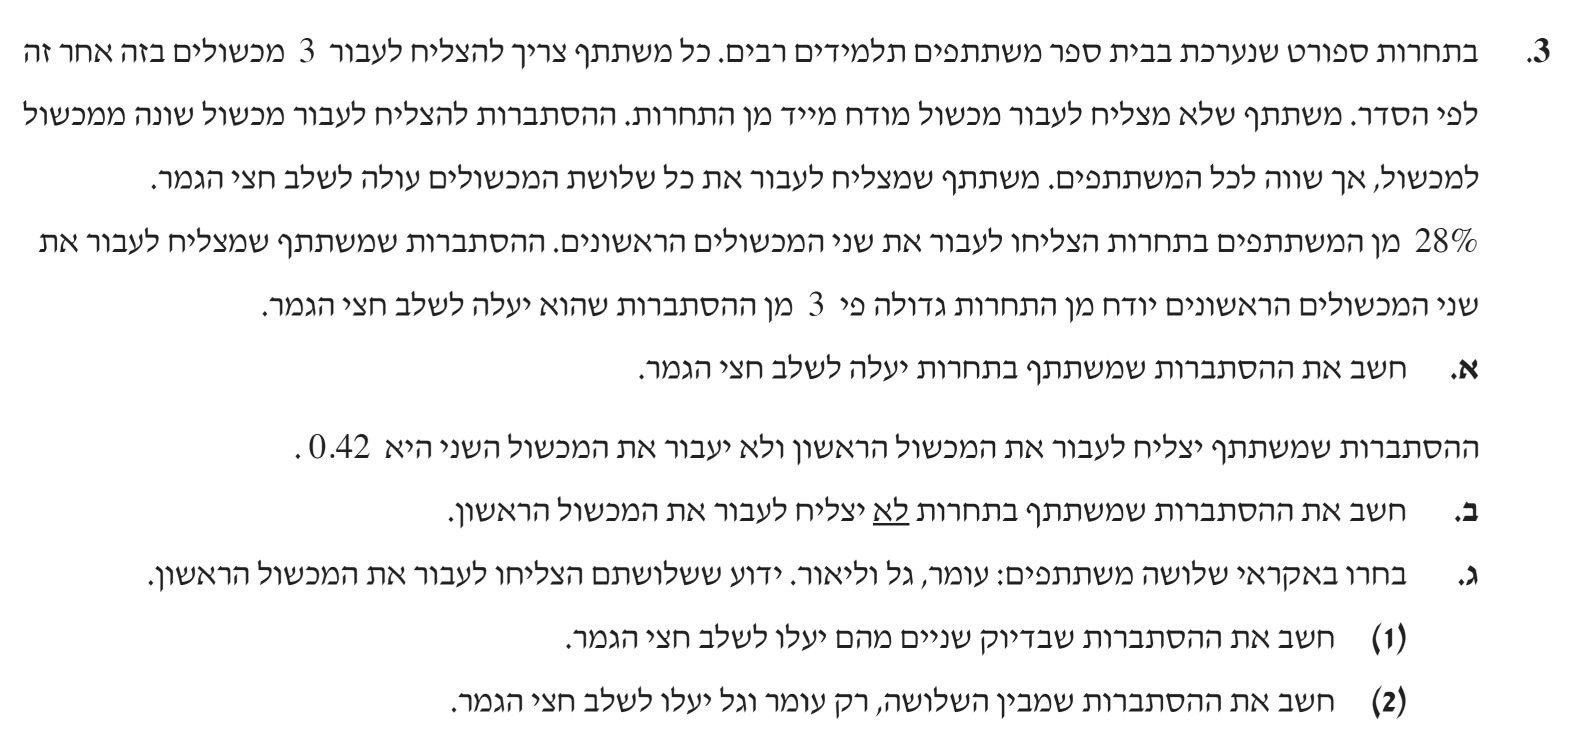
\includegraphics[width=\textwidth]{summer-2021b-3}
\end{center}

נניח שההסתברויות לעבור כל מכשול בלתי-תלויות. נסמן ב-%
$M1, M2, M3$ \L{(mikhshol)}
את המאורעות של לעבור כל מכשול, ונסמן ב-%
$HG$ \L{(hatzi gmar)}
את המאורע לעלות לחצי הגמר.

\textbf{סעיף א}

נתון ש-%
$P(M1 \cap M2)=P(M1)P(M2)=0.28$.
נשים לב שאם משתתף עבר את שני המכשולים הראשונים, ההסתברות שהוא יעלה לחצי הגמר שווה להתסתברות שהוא יעבור את המכשולים שלישי. לכן ניתן לחשב את ההסתברות המבוקשת כך:
\begin{eqnarray*}
P(HG)&=& P(M1\cap M2 \cap M3) = P(M1)P(M2)P(M3)\\
P(\overline{HG})&=& P(M1\cap M2 \cap \overline{M3}) = P(M1)P(M2)P(\overline{M3})\\
P(M3)&=&3(1-P(M3))\\
P(M3)&=&0.25\\
P(HG)&=&P(M1)P(M2)P(M3)=0.28\cdot 0.25=0.07\,.
\end{eqnarray*}

\textbf{סעיף ב}

נתון
$P(M1)P(\overline{M2})=0.42$
שמצטרף לנתון
$P(M1)P(M2)=0.28$.
ביחד:
\begin{eqnarray*}
P(M1)P(\overline{M2})&=&0.42\\
P(M1)P(M2)&=&0.28\\
P(M1)&=&0.42+0.28=0.70\\
P(\overline{M1})&=&0.30\,,
\end{eqnarray*}
כאשר אנו משתמש ב-%
$P(M2)+P(\overline{M2})=1$.

\textbf{סעיף ג 1}

ההסתברות של משתתף אחד לעלות לחצי הגמר היא:
\[
P(HG/M1)=\frac{P(HG\cap M1)}{P(M1)}=\frac{P(HG)}{P(M1)}=
\frac{0.07}{0.70}=0.01\,,
\]
כאשר אנו משתמשים ב-%
$M1 \subseteq HG$
כי משתתף עולה לחצי הגמר רק אם רק עובר את המכשול הראשון.

נסמן ב-%
$HG3/M13$
את ההסתברות המבוקשת. המילה "בדיוק" מכוון לנוסחת ברנולי, לכן:
\[
P(HG3/M13)={3\choose 2}\left(0.10\right)^2\left(0.90\right)^1=0.027\,.
\]

\textbf{סעיף ג 2}

נסמן ב-%
$O,G,L$
את המאורע שעומר, גל וליאור יעלו לחצי הגמר. השאלה שואלת על שני משתתפים מסויימים מתוך שלושה שנבחרו באקראי, ולכן אין צורך לצרף
${3\choose 2}$
לחישוב ההסתברות:
\[
P(O\cap G \cap \overline{L}) = P(O)P(G)P(\overline{L}) =
\left(0.10\right)\left(0.90\right)\left(0.10\right)=0.009\,.
\]

%%%%%%%%%%%%%%%%%%%%%%%%%%%%%%%%%%%%%%%%%%%%%%%%%%%%%%%%%%%%%

\newpage

\section{קיץ תשפ"א מועד א}

\begin{center}
\selectlanguage{english}
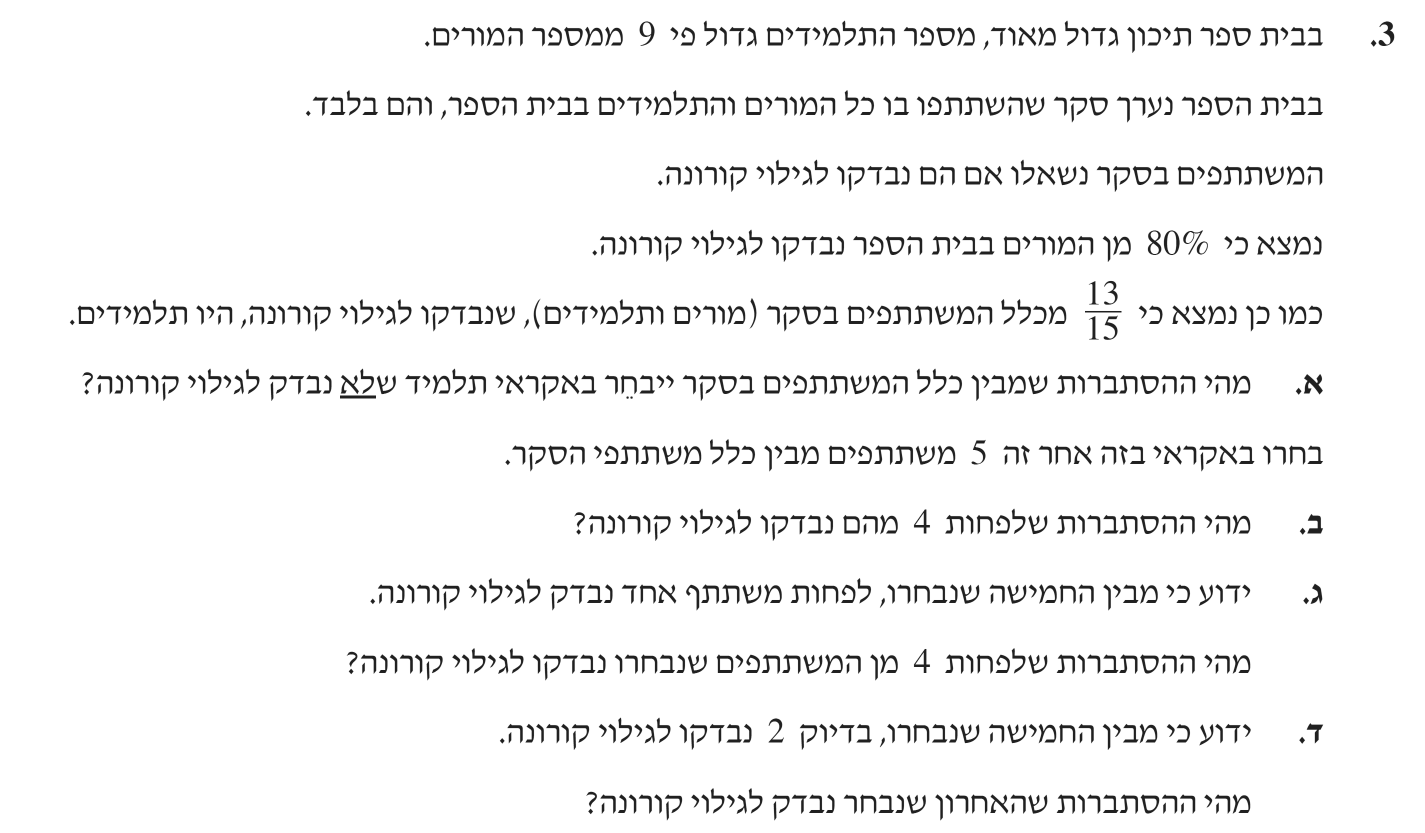
\includegraphics[width=.9\textwidth]{summer-2021a-3}
\end{center}

%%%%%%%%%%%%%%%%%%%%%%%%%%%%%%%%%%%%%%%%%%%%%%%%%%%%%%%%%%%%%

\section{קיץ תשפ"א מועד מיוחד}

\begin{center}
\selectlanguage{english}
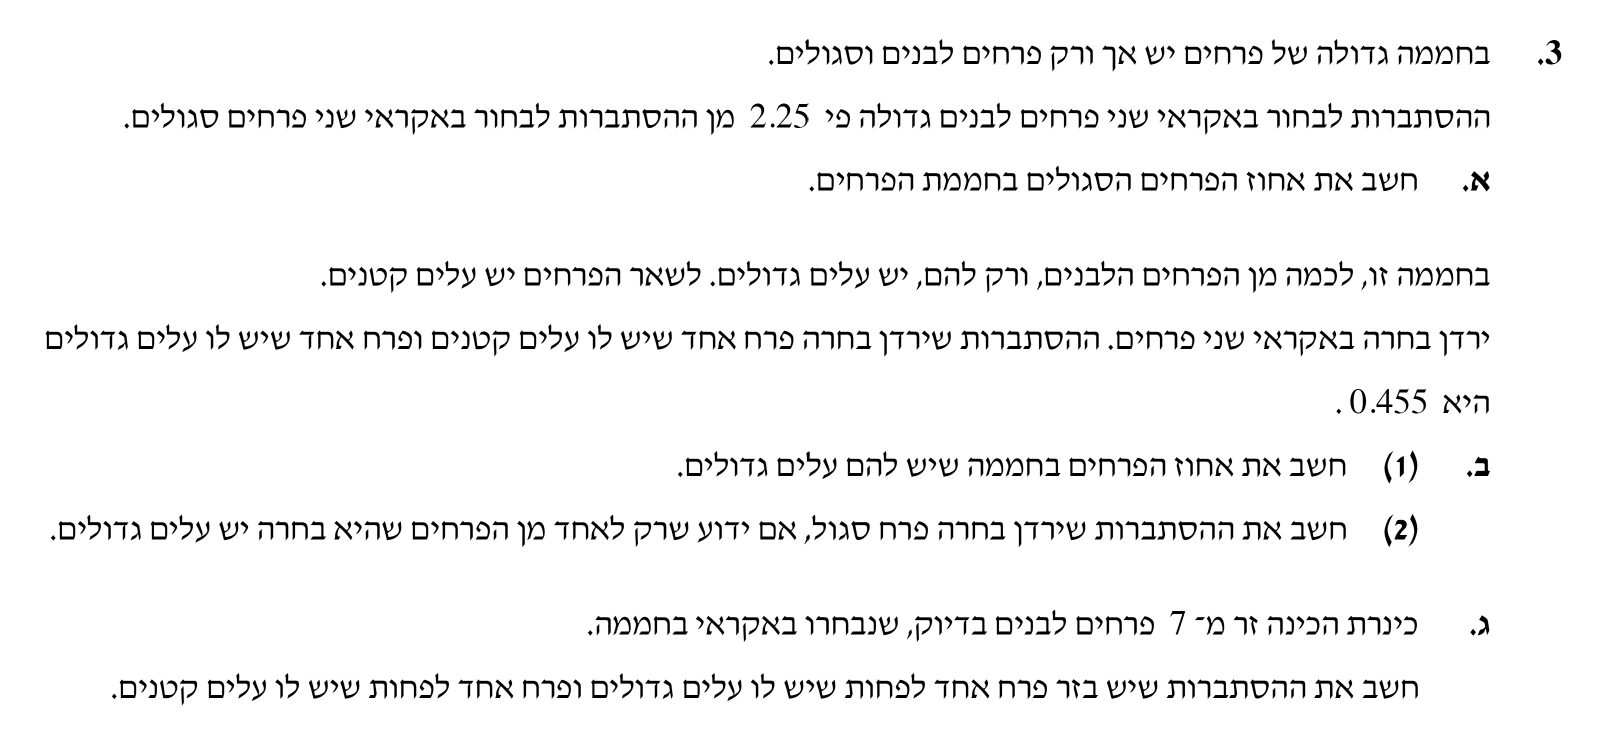
\includegraphics[width=.9\textwidth]{summer-2021sp-3}
\end{center}

%%%%%%%%%%%%%%%%%%%%%%%%%%%%%%%%%%%%%%%%%%%%%%%%%%%%%%%%%

\section{חורף תשפ"א}

\begin{center}
\selectlanguage{english}
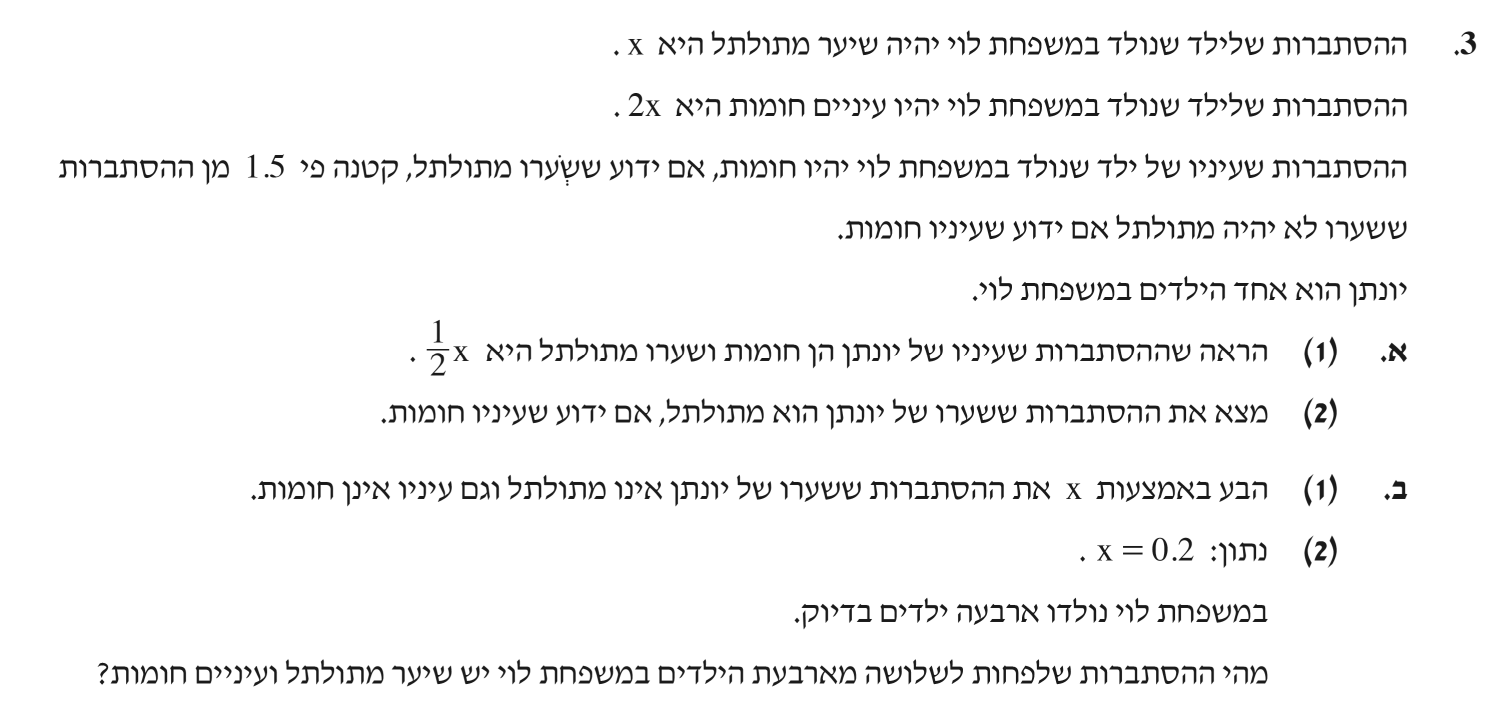
\includegraphics[width=.85\textwidth]{winter-2021-3}
\end{center}

%%%%%%%%%%%%%%%%%%%%%%%%%%%%%%%%%%%%%%%%%%%%%%%%%%%%%%%%%

\section{חורף תשפ"א מועד נבצרים}

\begin{center}
\selectlanguage{english}
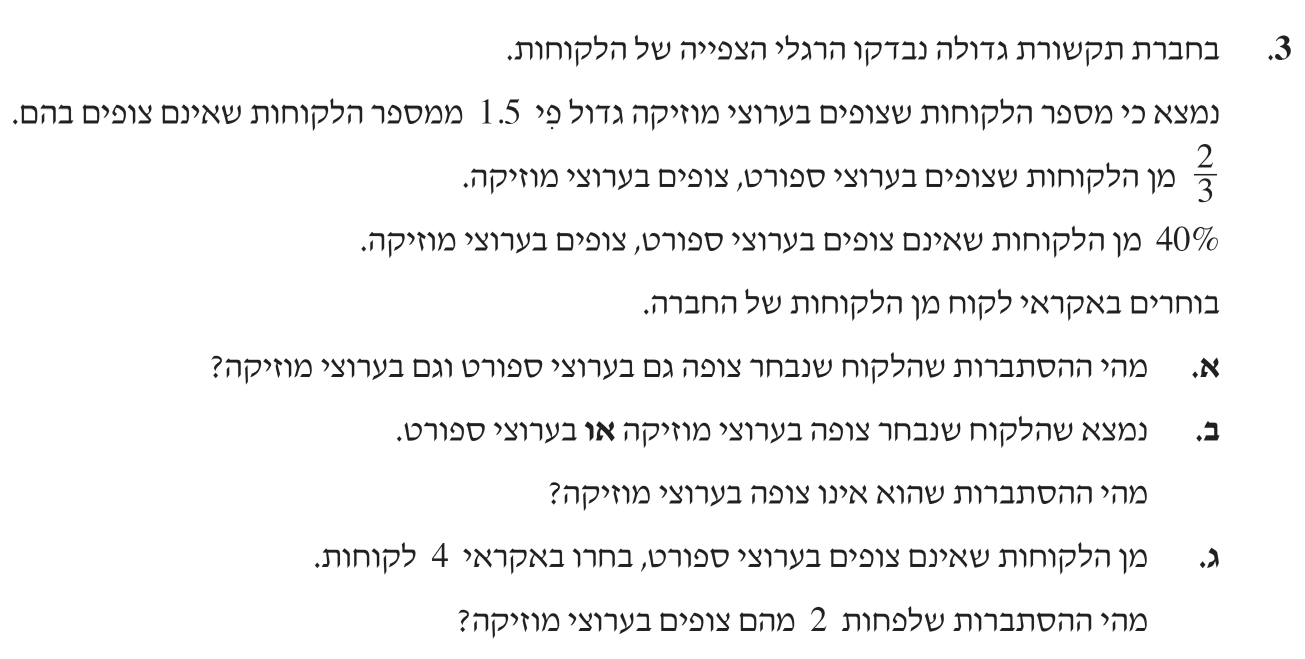
\includegraphics[width=.85\textwidth]{winter-2021nv-3}
\end{center}
